        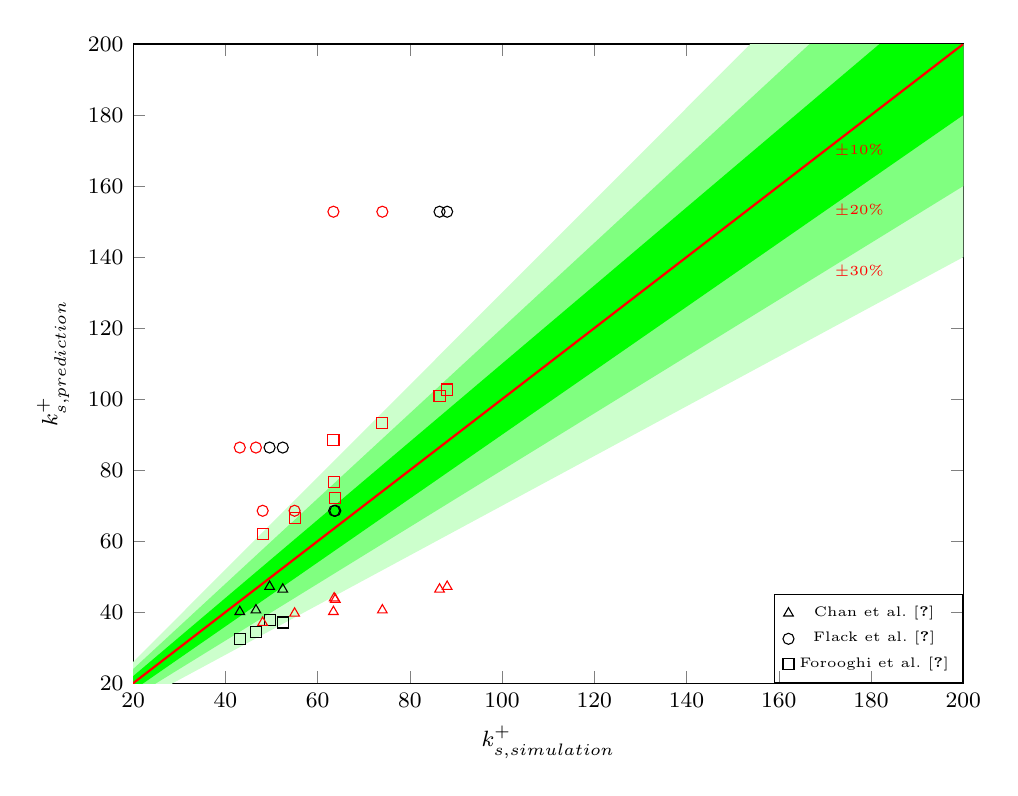
\begin{tikzpicture}[]
        \centering
        \begin{axis}[
            ylabel={$k_{s,prediction}^+$},
            xlabel={$k_{s,simulation}^+$},
            ymin=20, ymax=200,
			xmax=200,
			xmin=20,
			%xtick={-2,-1.5,...,-0.4},
            width=\linewidth,
            height=.8\linewidth,
            label style={font=\footnotesize},
			legend style={font=\tiny,at={(1,0)},anchor=south east,fill=none},
            tick label style={font=\footnotesize}
            ]
			 \fill[color=green!20,opacity=20] (0,0) -- (200,260) -- (200,140) -- cycle;
			 \fill[color=green!50,opacity=50] (0,0) -- (200,240) -- (200,160) -- cycle;
			 \fill[color=green!100,opacity=100] (0,0) -- (200,220) -- (200,180) -- cycle;

			\addplot [
            black,only marks,mark=triangle,
            ]
            coordinates{
                        (49.60,47.24)
            (52.46,46.47)
            (46.64,40.60)
            (43.14,40.14)
            };
			\addlegendentry{Chan et al.~\cite{chan_macdonald_chung_hutchins_ooi_2015}}
			\addplot [
            black,only marks,mark=o,
            ]
            coordinates{
            (63.60, 68.58)
            (63.85, 68.58)
            (88.10,152.78)
            (86.45,152.78)
            (49.60,86.38)
            (52.46,86.38)
            };
			\addlegendentry{Flack et al.~\cite{Flack2020}}
			\addplot [
            black,only marks,mark=square,
            ]
            coordinates{
            (49.60,37.78)
            (52.46,37.12)
            (46.64,34.36)
            (43.14,32.56)
            };
			\addlegendentry{Forooghi et al.~\cite{10.1115/1.4037280}}
			\addplot [
            red,only marks,mark=o,
            ]
            coordinates{
            (55.02,68.58)
            (48.10,68.58)
            (74.05,152.78)
            (63.44,152.78)
            (46.64,86.38)
            (43.14,86.38)
            };
			\addplot [
            red,only marks,mark=square,
            ]
            coordinates{
            (63.60, 76.62)
            (63.85, 72.16)
            (55.02,66.55)
            (48.10,62.12)
            (88.10,102.71)
            (86.45,100.92)
            (74.05,93.39)
            (63.44,88.52)
            };
			\addplot [
            red,only marks,mark=triangle,
            ]
            coordinates{
            (63.60, 43.98)
            (63.85, 43.61)
            (55.02,39.70)
            (48.10,37.10)
            (88.10,47.24)
            (86.45,46.47)
            (74.05,40.60)
            (63.44,40.14)

            };
						\addplot [
            red,thick,solid,mark=square,
            ]
            coordinates{
            (0, 0)
            (201, 201)
            };
			\node[red,right] at (axis cs: 170,170) {\tiny $\pm10\%$};
						\node[red,right] at (axis cs: 170,153) {\tiny $\pm20\%$};
									\node[red,right] at (axis cs: 170,136) {\tiny $\pm30\%$};
        \end{axis}
        \end{tikzpicture}